\documentclass[10pt]{article}
\usepackage[margin=0.72in]{geometry}
\usepackage{amsmath,amssymb,booktabs,graphicx,microtype,hyperref,xcolor,array,enumitem,caption}
\usepackage[T1]{fontenc}
\usepackage{lmodern}
\usepackage{float}
\graphicspath{{../figures/}}
\hypersetup{colorlinks=true,linkcolor=blue!55!black,citecolor=blue!55!black,urlcolor=blue!55!black}
\captionsetup{font=small,labelfont=bf}
\setlist{nosep,leftmargin=*}

\title{\textbf{AstraBuild: GPT-6 Astra as a Long-Horizon 3D Engineering Agent\\for Component-Level Substation Reconstruction}}
\author{Project Team\\\small Draft authorship placeholder}
\date{Advisor-discussion draft v0.7 --- 16 September 2026}

\newcommand{\scopewarning}{\textbf{Scope note:} all centimeter-scale surface residuals reported here are comparisons to the same photogrammetric coarse mesh used by the modeling workflow; they are \emph{not} independent survey accuracy.}
\newcommand{\researchq}[1]{\paragraph{#1}}

\begin{document}
\maketitle

\begin{abstract}
Can a general-purpose reasoning agent turn noisy photogrammetric geometry, heterogeneous field images, and engineering records into an editable component-level digital twin over a long tool-use horizon? We study this question through a longitudinal reconstruction of a 220~kV operating substation. AstraBuild treats reconstruction as an evidence-grounded closed loop: selected coarse geometry, field photographs, engineering records, and persistent history are compiled for a reasoning agent; the agent proposes Blender/Python operations; deterministic tools materialize those operations; layered validation returns structured feedback; and the result, failure, limitation, or human correction is retained for subsequent iterations. The core record contains 38 reconstruction batches through D38, followed by a geometry-preserving material layer (D40) and an inspection-semantic augmentation (D41). At the D38.2/D40-equivalent geometry scale, the project contains 37,153 objects, 755 scenes, 858 collections, and 3,916 mesh datablocks. A 1,550-record surface-comparison ledger has median/p90/p95 residuals of 0.036/0.084/0.116~m. \scopewarning{} A selected coverage audit reduces the high-region fraction farther than 1~m from modeled geometry from 78.8\% to 14.6\%. The record also preserves failures that alter later measurement, component abstraction, and human-feedback protocols. D41 finally aligns 79 accessory meshes spanning 17 inspection-relevant part classes into a shared transformer accessory layer instantiated for T1 and T2. The contribution is not a claim of fully autonomous or survey-grade reconstruction, but an auditable pattern for using a general-purpose reasoning model as a long-horizon reconstruction operator bounded by explicit evidence, deterministic tooling, immutable history, and layered verification.
\end{abstract}

\paragraph{Experiment provenance.}
The project owner reports the configuration as \textbf{Codex + GPT-6 Astra with Extra High reasoning}. The inspected historical Blender batch records do not embed model/reasoning-effort metadata. This setting is therefore marked as user-confirmed rather than independently recovered from the old logs.

\section{Introduction}
Photogrammetry and neural view-synthesis methods can recover impressive scene geometry and appearance~\cite{schonberger2016sfm,mildenhall2020nerf,kerbl2023gaussians}. Industrial digital twins, however, often require a different representation: editable devices, reusable component families, explicit connectors and hierarchy, semantic identity, and traceable revision history. A fused surface does not by itself identify which repeated structures should share one master asset, how a transformer inspection point maps to a visible part, or whether a later correction silently invalidated previous work.

The Xialin reconstruction starts from a registered but noisy photogrammetric mesh, UAV/ground imagery, engineering inventories, semantic records, manual position proxies, and human review. These sources play different epistemic roles. Coarse geometry constrains layout and reveals occupied regions; imagery constrains visible component form; inventories constrain expected semantics; human feedback identifies errors or authorizes equivalence; and persistent batch artifacts record what the system previously believed.

General-purpose model work in robotics provides a useful conceptual precedent. Code as Policies and VoxPoser expose executable/spatial interfaces~\cite{liang2023code,huang2023voxposer}; GPT-Policy separates context construction, fixed-model tool selection, constrained execution, and feedback-driven replanning~\cite{cheng2026gptpolicy}; and the GPT-6 Astra embodied-policy report studies a System-2 role for semantic reasoning and exception handling~\cite{su2026astraembodied}. We ask an analogous question for 3D engineering: can a general-purpose model operate a reconstruction process while deterministic geometry code and validators remain the acceptance authority?

This paper is a \emph{longitudinal single-site case study}, not an IID benchmark. Its evidence is therefore a combination of artifact structure, metric ledgers, preserved failures, protocol changes, human-feedback traces, and semantic augmentation rather than one success rate.

\subsection{Research questions}
\researchq{RQ1 --- Structured reconstruction.} Can coarse geometry, images, and records become an editable component-level scene with reusable equipment families?
\researchq{RQ2 --- Verifier-bounded reliability.} Can explicit validation expose invalid hypotheses and force geometric, metric, or abstraction revisions rather than silent acceptance?
\researchq{RQ3 --- Coverage-driven completion.} Can residual/occupancy audits identify missing geometry that inventory-driven completion misses?
\researchq{RQ4 --- Human-steerable correction.} Can sparse human spatial feedback be translated into traceable 3D corrections without direct vertex-level modeling?
\researchq{RQ5 --- Inspection semantics.} Can stabilized geometry gain inspection-addressable parts while preserving prior history?

\subsection{Contributions}
We contribute: (1) an evidence-grounded 3D-engineering-agent formulation with a canonical reconstruction core and task-specific engineering operators; (2) a heterogeneous task suite from one operating industrial site; (3) intermediate engineering evidence---profiles, preflight diagnostics, route fits, clean/overlay/reference reviews, validators, manifests and retained revisions---as a first-class record of the reconstruction trajectory; (4) failure/recovery studies showing revisions to metrics, representation choices, reusable-asset boundaries, task selection and feedback interpretation; and (5) a station-scale compositional demonstration with a later inspection-semantic layer.

\section{Related Work}
\paragraph{Surface reconstruction.} Classical structure-from-motion/photogrammetry~\cite{schonberger2016sfm}, NeRF~\cite{mildenhall2020nerf}, and 3D Gaussian Splatting~\cite{kerbl2023gaussians} provide increasingly powerful geometry/appearance representations. Our focus is downstream: converting incomplete spatial/image evidence into editable and semantically addressable engineering structure.

\paragraph{Programmatic 3D and tool-using agents.} Programmatic embodied control~\cite{liang2023code}, 3D language-conditioned objectives~\cite{huang2023voxposer}, and VLA systems~\cite{brohan2023rt2} demonstrate the value of structured action interfaces. 3D-GPT decomposes procedural 3D generation into task-dispatch, conceptualization and modeling agents~\cite{sun2023threegpt}; SceneCraft constructs scene graphs, translates spatial relations into Blender-executable code, visually reviews renders and distills reusable functions~\cite{hu2024scenecraft}. AstraBuild differs in problem direction: it reverse-engineers registered physical evidence and therefore relies on metric profiles, route/topology fits, explicit validation domains, history preservation and retained failures. GPT-Policy and the Astra embodied-policy report are particularly relevant in separating context, reasoning, constrained execution and feedback, and in organizing one shared architecture across heterogeneous tasks~\cite{cheng2026gptpolicy,su2026astraembodied}. RoboDojo illustrates benchmark-style metric breakdowns~\cite{chen2026robodojo}; AstraBuild borrows the reporting discipline but does not claim an IID benchmark.

\section{Problem Formulation}
Let the persistent reconstruction state be
\begin{equation}
S_t=(M_t,A_t,X_t,Q_t),
\end{equation}
where $M_t$ is scene geometry, $A_t$ reusable asset hierarchy, $X_t$ semantic/inspection mappings, and $Q_t$ provenance/validation records. A bounded context is compiled as
\begin{equation}
C_t=\mathcal{C}(G,I,R,U,H_t),
\end{equation}
from coarse geometry $G$, images $I$, engineering records $R$, manual spatial priors $U$, and persistent history $H_t$. The model proposes
\begin{equation}
a_t\sim\pi_\theta(\cdot\mid C_t,S_t,f_{t-1}),
\end{equation}
then deterministic execution and validation produce
\begin{equation}
(\widetilde S_{t+1},e_t)=E(a_t,S_t),\qquad v_t=V(\widetilde S_{t+1},G,Q_{\le t}).
\end{equation}
Only artifacts satisfying the relevant batch checks are promoted into the next persistent state; otherwise diagnostic evidence is retained for replanning.

\begin{figure}[H]
\centering
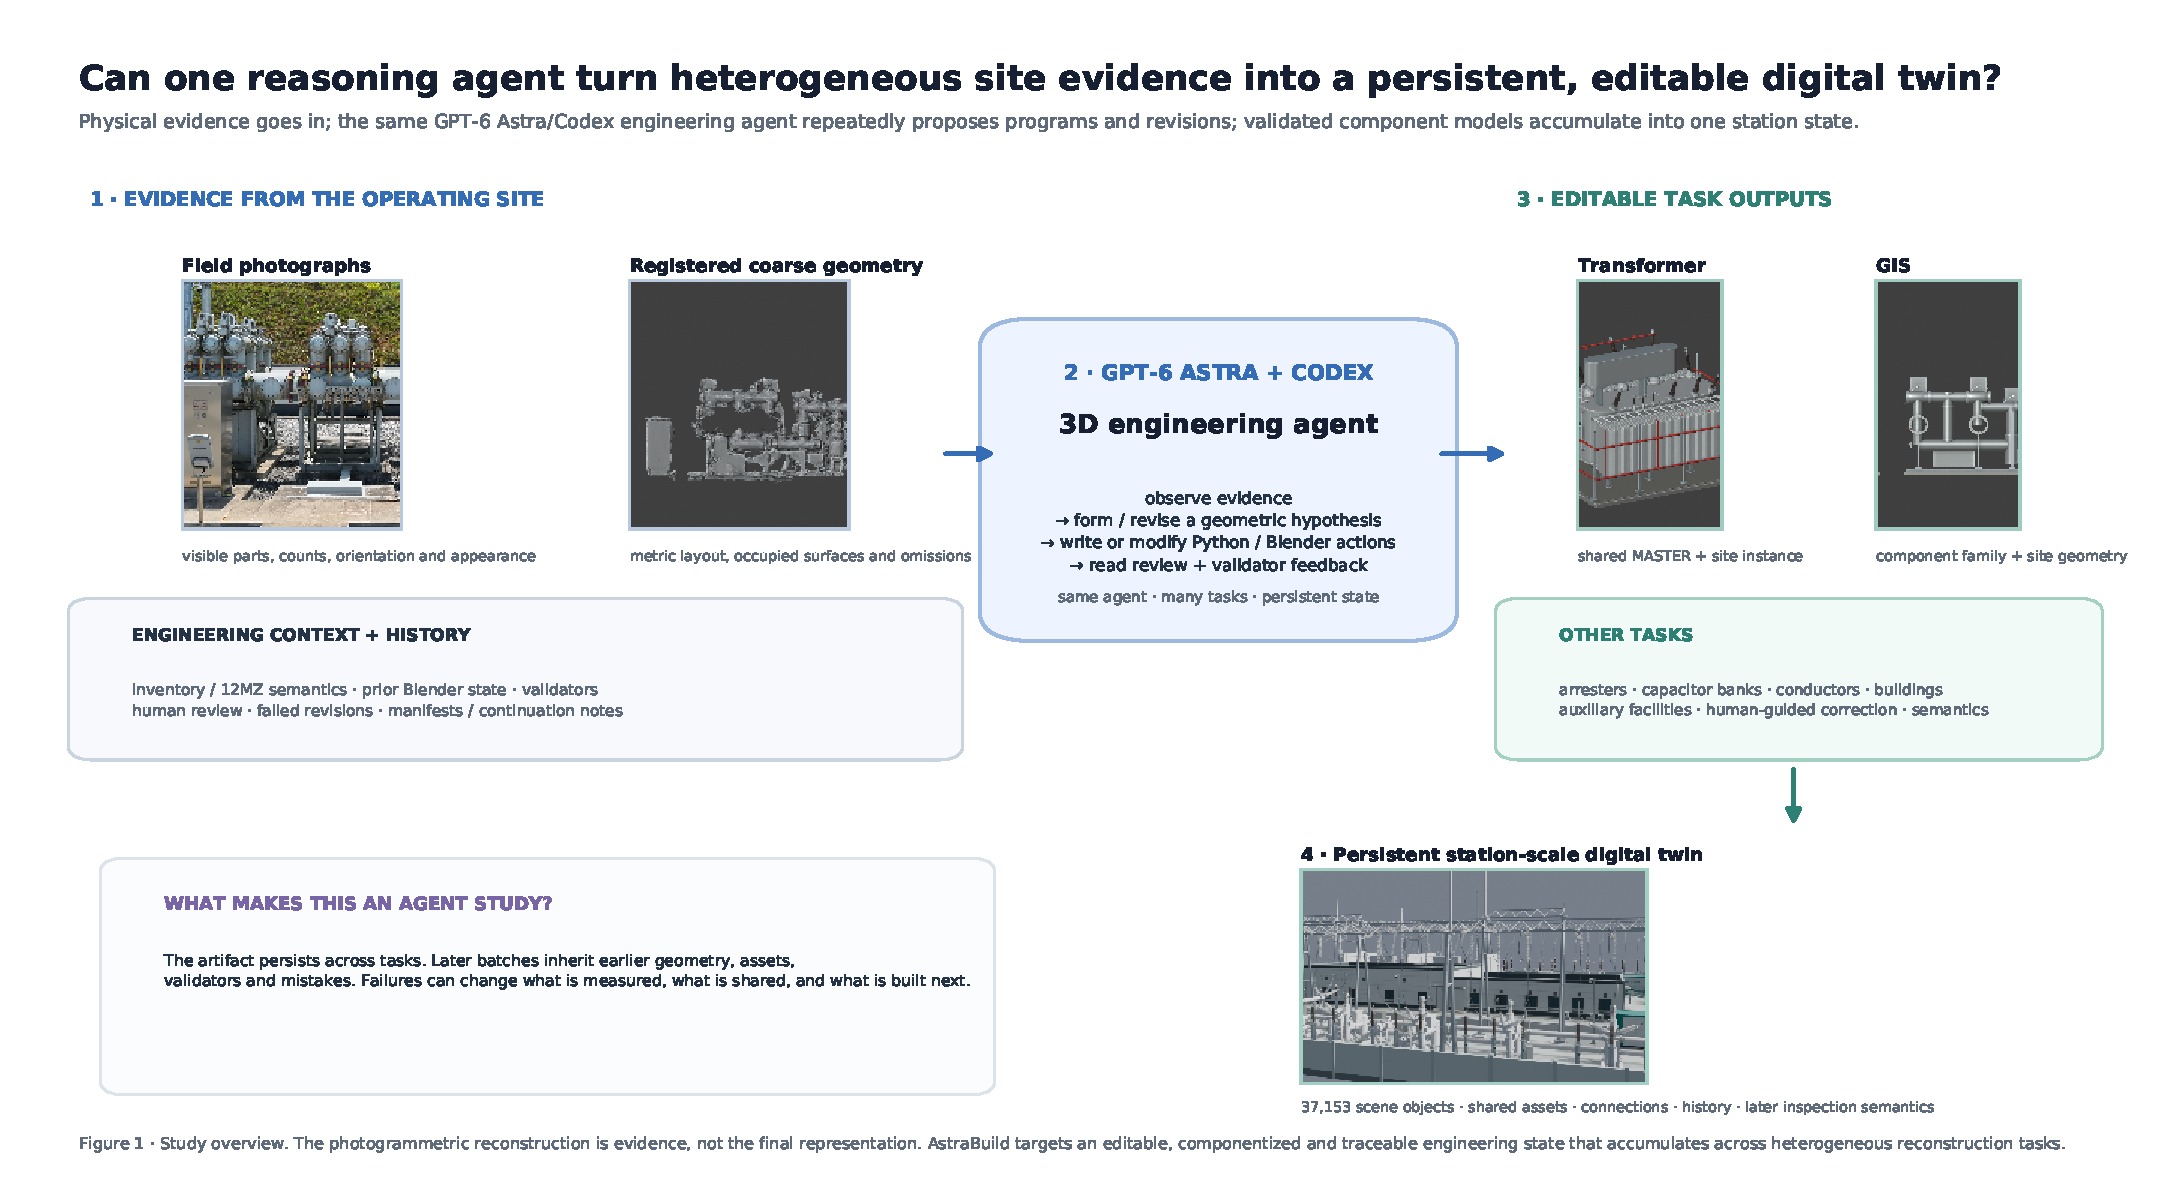
\includegraphics[width=\linewidth]{fig01_agentic_loop.pdf}
\caption{Study overview. Field imagery, registered coarse geometry, engineering records, and prior history form the evidence context. The same Astra/Codex engineering agent repeatedly proposes and revises programs; validated component models accumulate into one editable station state.}
\label{fig:loop}
\end{figure}

\section{Study Materials and Provenance}
\subsection{Evidence sources}
\begin{table}[H]
\centering
\caption{Primary evidence sources and their epistemic role.}
\small
\begin{tabular}{p{0.22\linewidth}p{0.21\linewidth}p{0.28\linewidth}p{0.23\linewidth}}
\toprule
Source & Recorded scale & Role & Boundary \\
\midrule
Photogrammetric coarse mesh & 23 tiles, $\sim$112$\times$134 m & layout, local surface reference, omission discovery & not independent truth for residuals using the same mesh \\
UAV/ground images & 775 early identity-photo candidates + later audits & visible form, count, ordering, materials & incomplete calibration/identity in several stages \\
Inventory + 12MZ & 153 devices, 106 names, 1,842 rows & expected semantics, codes, inspection concepts & inventory presence does not prove geometry completion \\
UE/manual boxes & 82 & position prior, cross-check & not an independently surveyed reference \\
Human review + batch history & 38 core batches + revisions & error signals, equivalence authorization, external memory & human intervention is part of the method \\
\bottomrule
\end{tabular}
\end{table}

\subsection{Version boundary}
D38.2 is the headline core-geometry baseline. D40 changes material assignment while validating geometry/transform invariance. D41 is an additive transformer inspection-semantic/accessory layer and the research endpoint. The paper keeps these scopes separate rather than reporting all numbers as one frozen artifact.

\section{AstraBuild Method}
\subsection{Evidence compiler}
Each batch reduces the raw repository into bounded evidence: marked images, local coarse-mesh crops, local-to-world transforms, source origins, device/inventory slices, prior manifests, review renders, failure notes, and user feedback. The goal is not maximal context length but preservation of task-relevant evidence and provenance.

\subsection{Asset--installation separation}
Early P-line experiments construct normalized photo-derived asset hypotheses, while B-line/site work uses local metric frames and coarse geometry for installation/reconstruction. Candidate assets are rejected when proportion/correspondence checks do not justify reuse. This separation prevents a visually plausible asset from automatically becoming site truth.

\subsection{Reusable masters and site instances}
Mature geometry is organized into shared \texttt{MASTER} collections, site instances, site-specific connectors, and review layers. Reuse encodes a falsifiable equivalence hypothesis: when field evidence shows a variant or finite site-specific segment, the abstraction is split rather than silently deforming a shared master.

\subsection{Immutable batch memory}
Later batches typically retain a continuation note, plan JSON, builder, independent validator, saved Blender/component outputs, manifests/validation JSON, and review media. Revisions create new paths; failed drafts and limitations remain in history.

\subsection{Worked example: B32 as an observable agent--tool trace}
A generic workflow is difficult to interpret without one complete task. B32 reconstructs the 110~kV and 220~kV secondary-equipment cabins and preserves the inherited state, measurement scripts, diagnostics, three revisions, componentized Blender output, fixed-camera review images, an interactive review page, validation, and continuation memory. The historical record does \emph{not} preserve GPT-6 Astra's private chain-of-thought; the analysis therefore reports the observable engineering decision trail rather than an inferred reasoning transcript.

\begin{figure}[H]
\centering
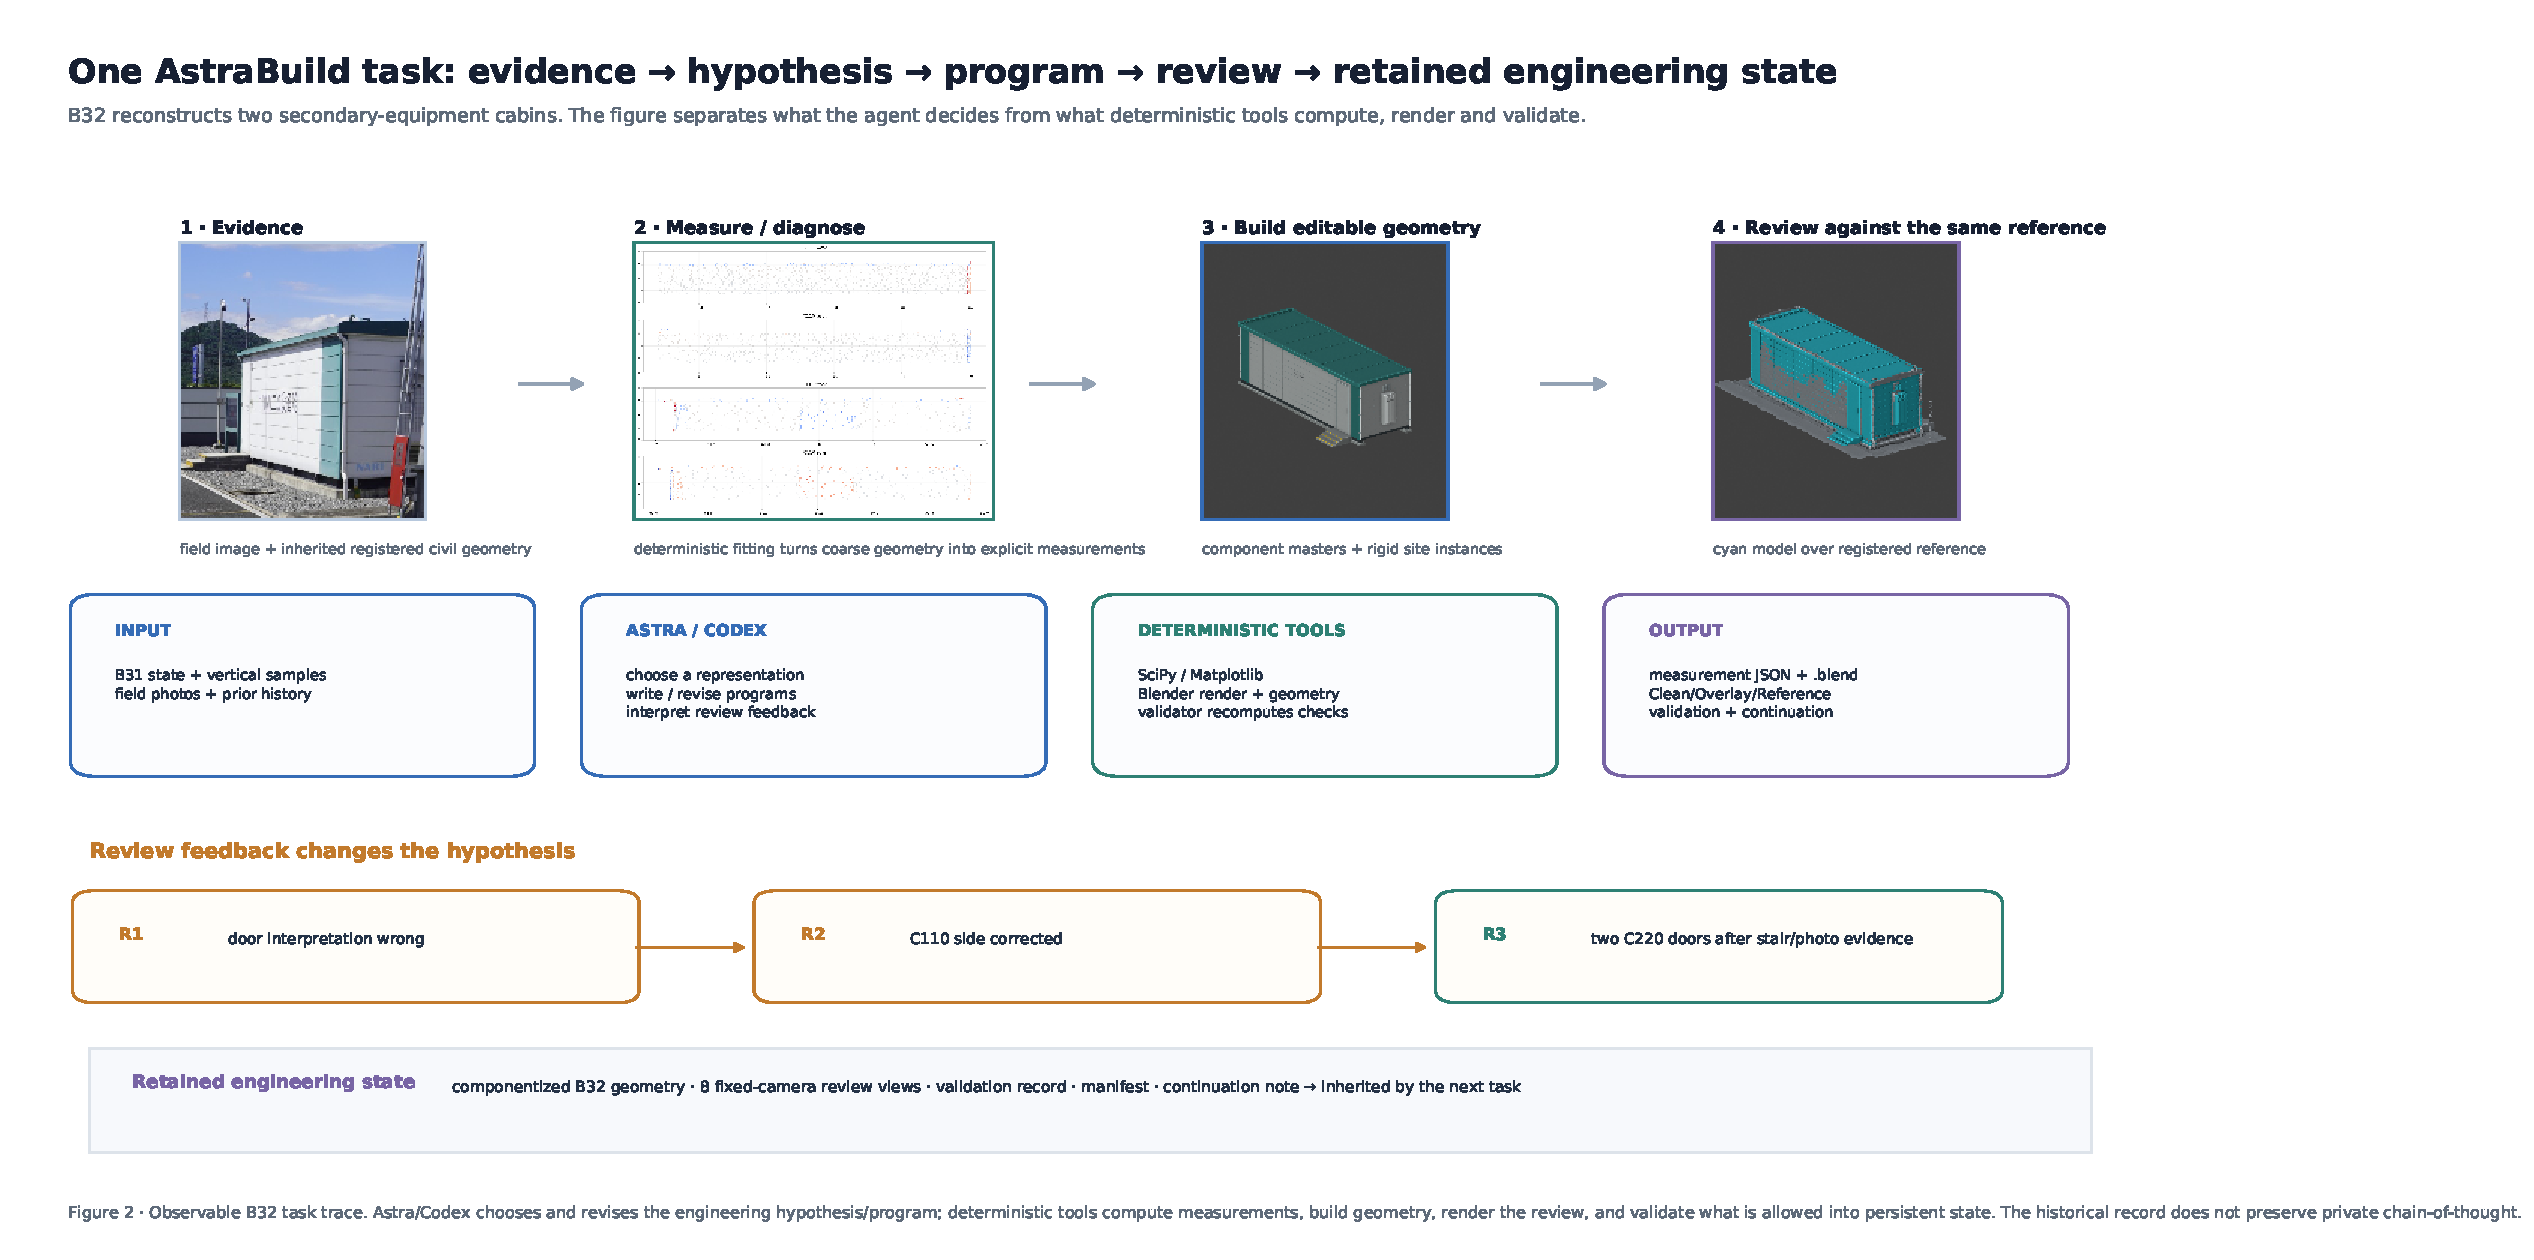
\includegraphics[width=\linewidth]{fig12_b32_worked_example.pdf}
\caption{One concrete reconstruction task. B32 turns field imagery and inherited registered civil geometry into an editable cabin model through an explicit evidence--hypothesis--program--review--validation trace. The figure separates agent decisions from deterministic computation, rendering, and validation.}
\label{fig:b32trace}
\end{figure}

The B32 evidence transformation is explicit. \texttt{B31\_vertical\_samples.npz} and the inherited station frame are processed by \texttt{measure\_B32\_containers.py}; a soft-L1 rectangular-wall fit writes \texttt{B32\_container\_measurements.json} plus C110/C220 facade diagnostics containing width, length, yaw and root transforms. A second evidence path uses low-height registered geometry and field photographs: \texttt{inspect\_B32\_steps.py} writes \texttt{B32\_source\_steps\_diagnostic.png}, which exposes staircase signatures used to correct the door interpretation.

This evidence changes the model, rather than merely illustrating it. R1 used one door per cabin and placed C110 on the west side. R2 moves the C110 door to the east. R3 places the C110 east door at local $Y\approx-3.90$ and two C220 west doors at approximately $-5.50$ and $+5.32$, clipping panels and seams around the openings. The continuation record explicitly rejects an earlier interpretation of a C220 middle depression after photographs and two stair-platform signatures contradict it.

\texttt{build\_B32\_r3.py} converts the accepted measurements into a shared end-wall/HVAC master, a shared door master, separate size-specific C110/C220 cabin masters and rigid SITE roots. It also creates eight fixed local cameras; each camera has Clean, Overlay and Reference variants. \texttt{review\_B32.py} packages these as the self-contained \texttt{B32\_review.html}: eight directions, three display states, a split slider, 25 embedded images and 27 recorded renders. \texttt{validate\_B32\_r3.py} then reopens the artifact and checks inherited-state preservation, fixed odd-triangle facade domains, door openings, stair elevations, camera framing and component-library round-trip. The final ledger records 34,191 inherited objects, 7,114 inherited station transforms and 2,953 protected prior files as preserved. These facade comparisons remain correlated photogrammetric-reference checks, not independent survey accuracy.

\subsection{Historical review protocol across device cases}
The review mechanism used in B32 is not exceptional. The publication catalog contains 32 formal batches with original \texttt{review.html} pages from B07 through D38. These pages were generated during the corresponding batch, embed actual Blender renders, and preserve the task-specific explanatory text and limitations. Across tasks, the recurring protocol is a named equipment/view selector plus fixed-camera model/reference evidence: Clean geometry, a model/reference Overlay or split-slider comparison, and Reference-only coarse geometry. B07 compares an earlier transformer candidate with the revised model; B08 switches between T1/T2; B09/B10 select individual capacitor-bank groups and expose Clean/Compare/Overlay/Reference modes; later GIS, conductor, civil and correction batches retain the same same-camera review principle.

\begin{figure}[H]
\centering
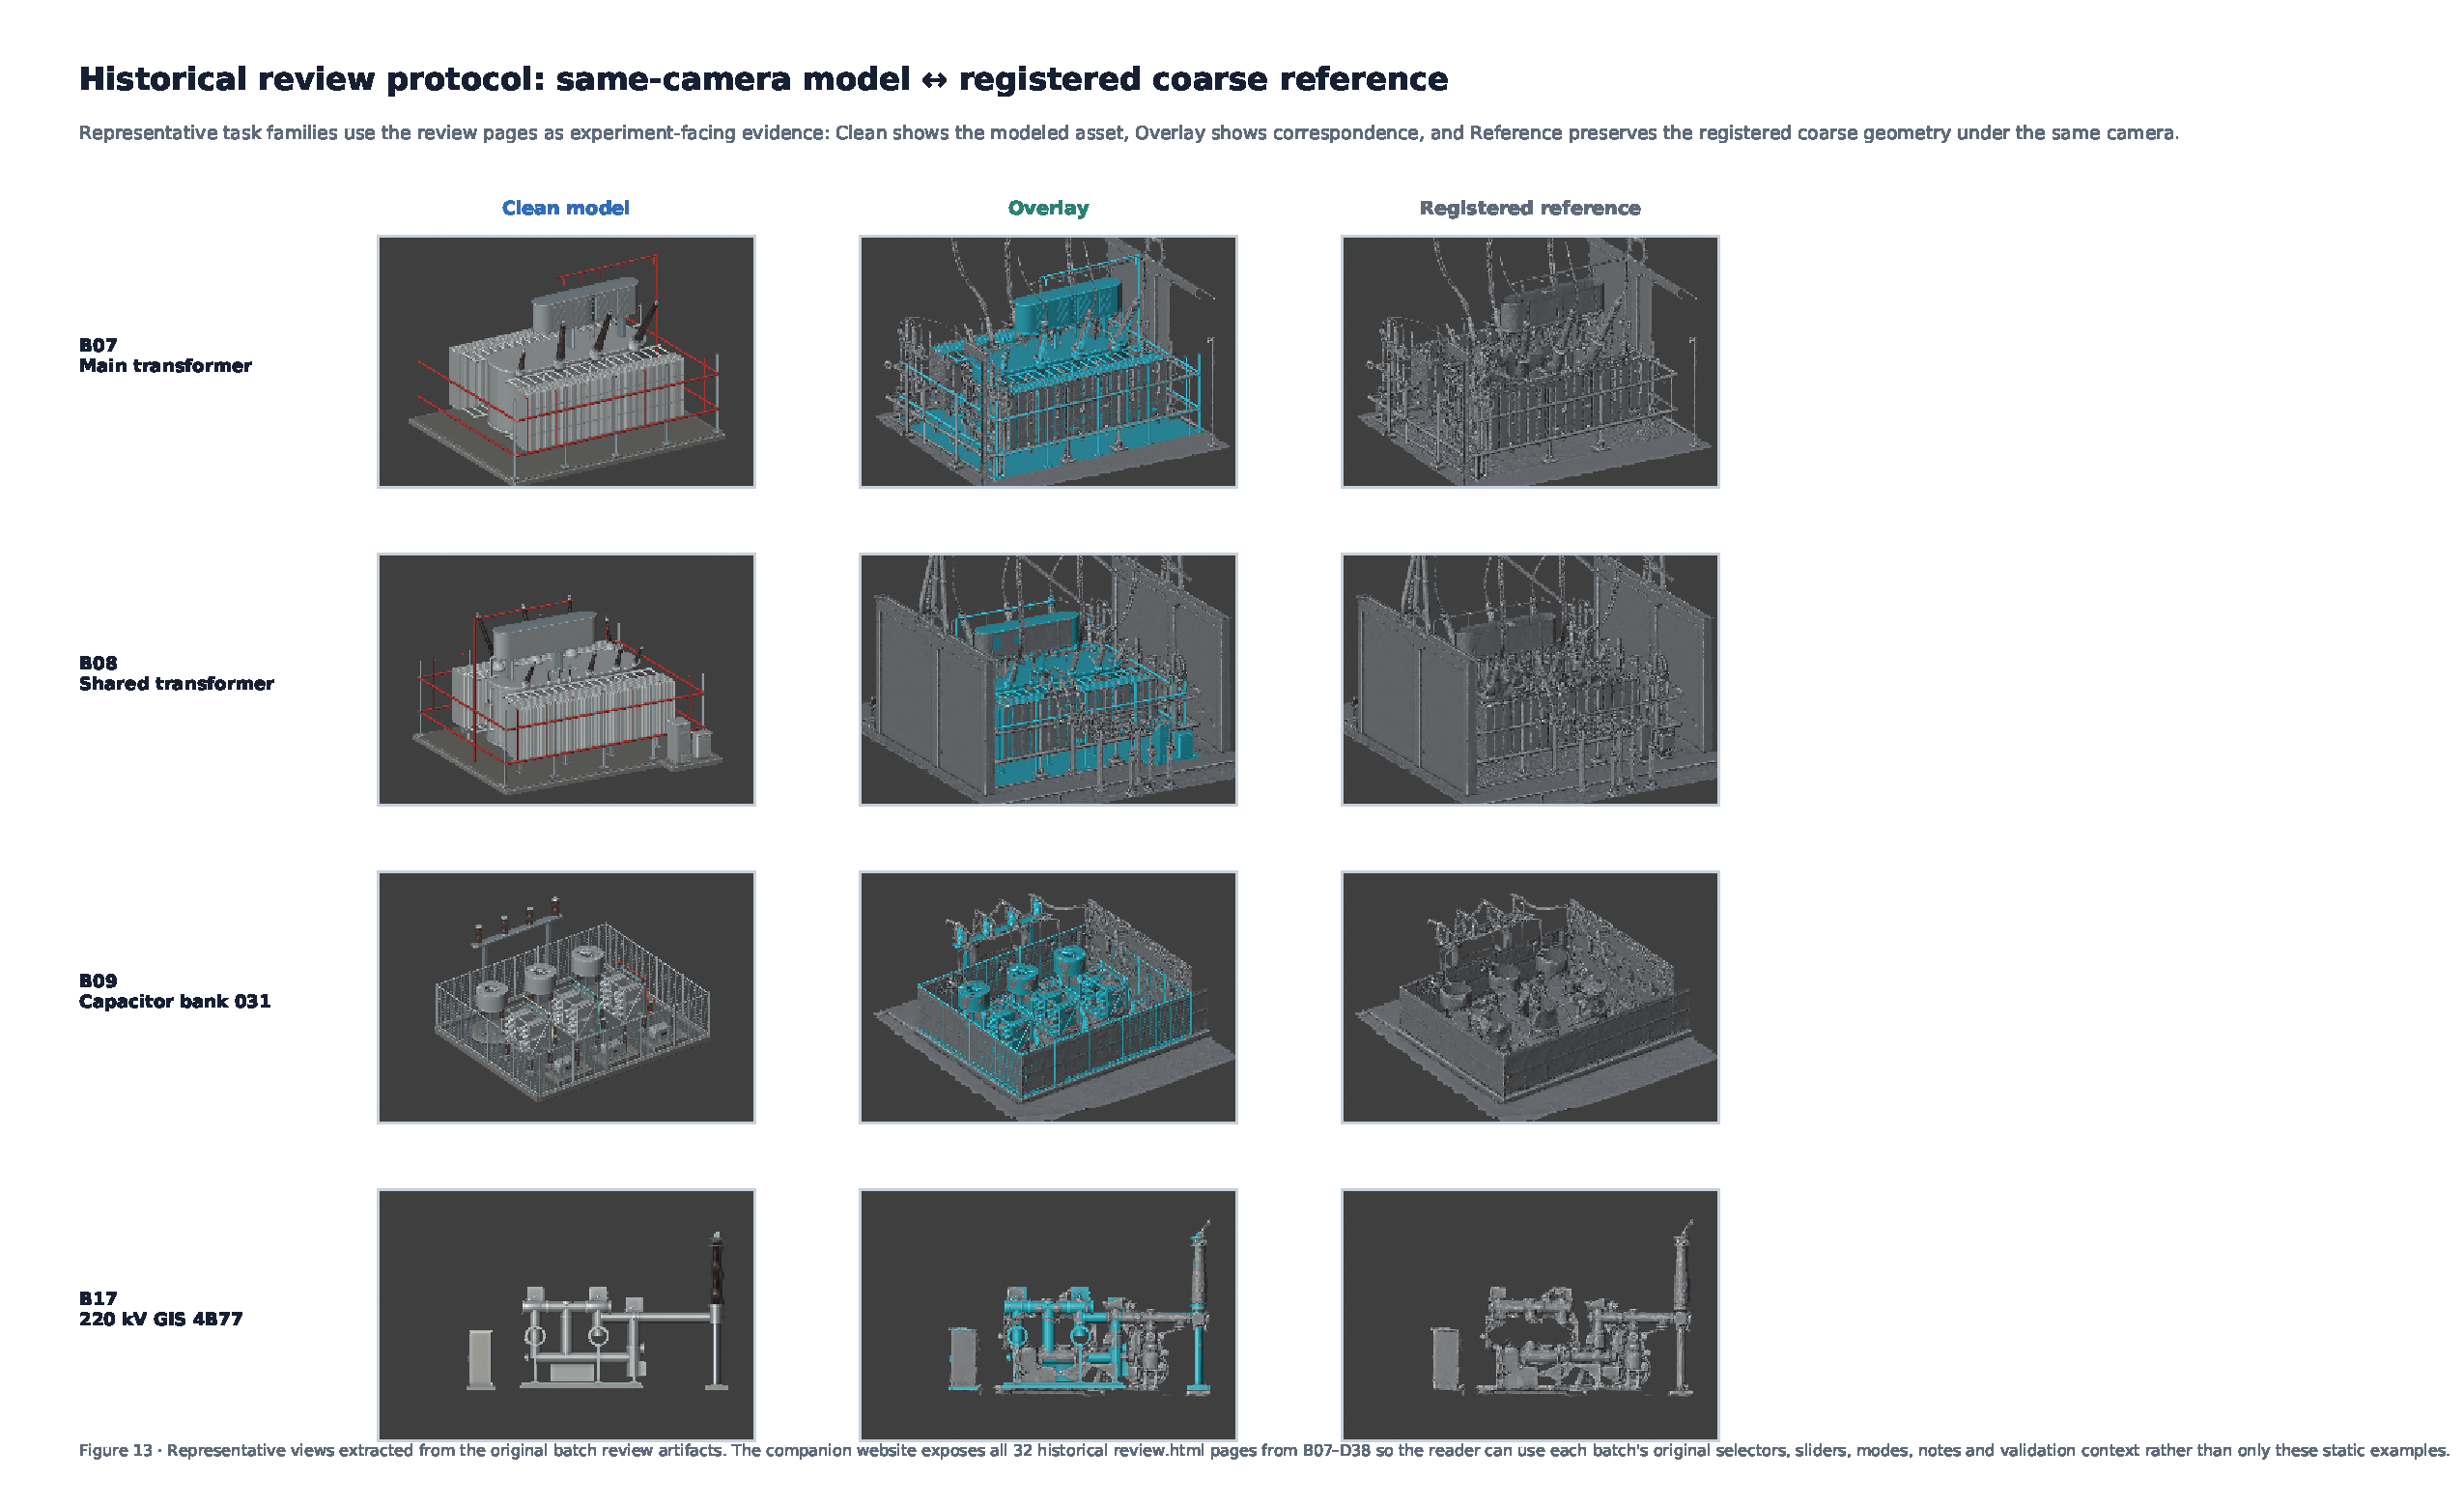
\includegraphics[width=\linewidth]{fig13_review_protocol.pdf}
\caption{Representative historical review triplets from B07, B08, B09 and B17. The companion website exposes all 32 original review pages rather than only these static samples.}
\label{fig:reviewprotocol}
\end{figure}

For the case-study interpretation of the experiment, this matters because a device task is not evidenced only by a final render. The reader can inspect the generated component geometry against the registered coarse reconstruction using the same batch-generated review interface. The review page forms the visual inspection layer of each task dossier; measurement/preflight/diagnostic artifacts precede it, while validation/manifests and continuation memory follow it.

\subsection{Generalizing from B32: canonical reconstruction loop and task-specific operators}
A filename-level audit of B01--B36 shows a stable core process---freeze/prepare inherited state, extract a registered local reference, inspect and plan, build/refine, render clean/overlay/reference review views, validate/audit, then freeze the release and continuation memory---but not one rigid identical pipeline. Measurement/profile fitting, representation preflight, conductor-route fitting, coverage audit, collision/interference checks and human-markup correction are activated only when the task or failure requires them.

\begin{figure}[H]
\centering
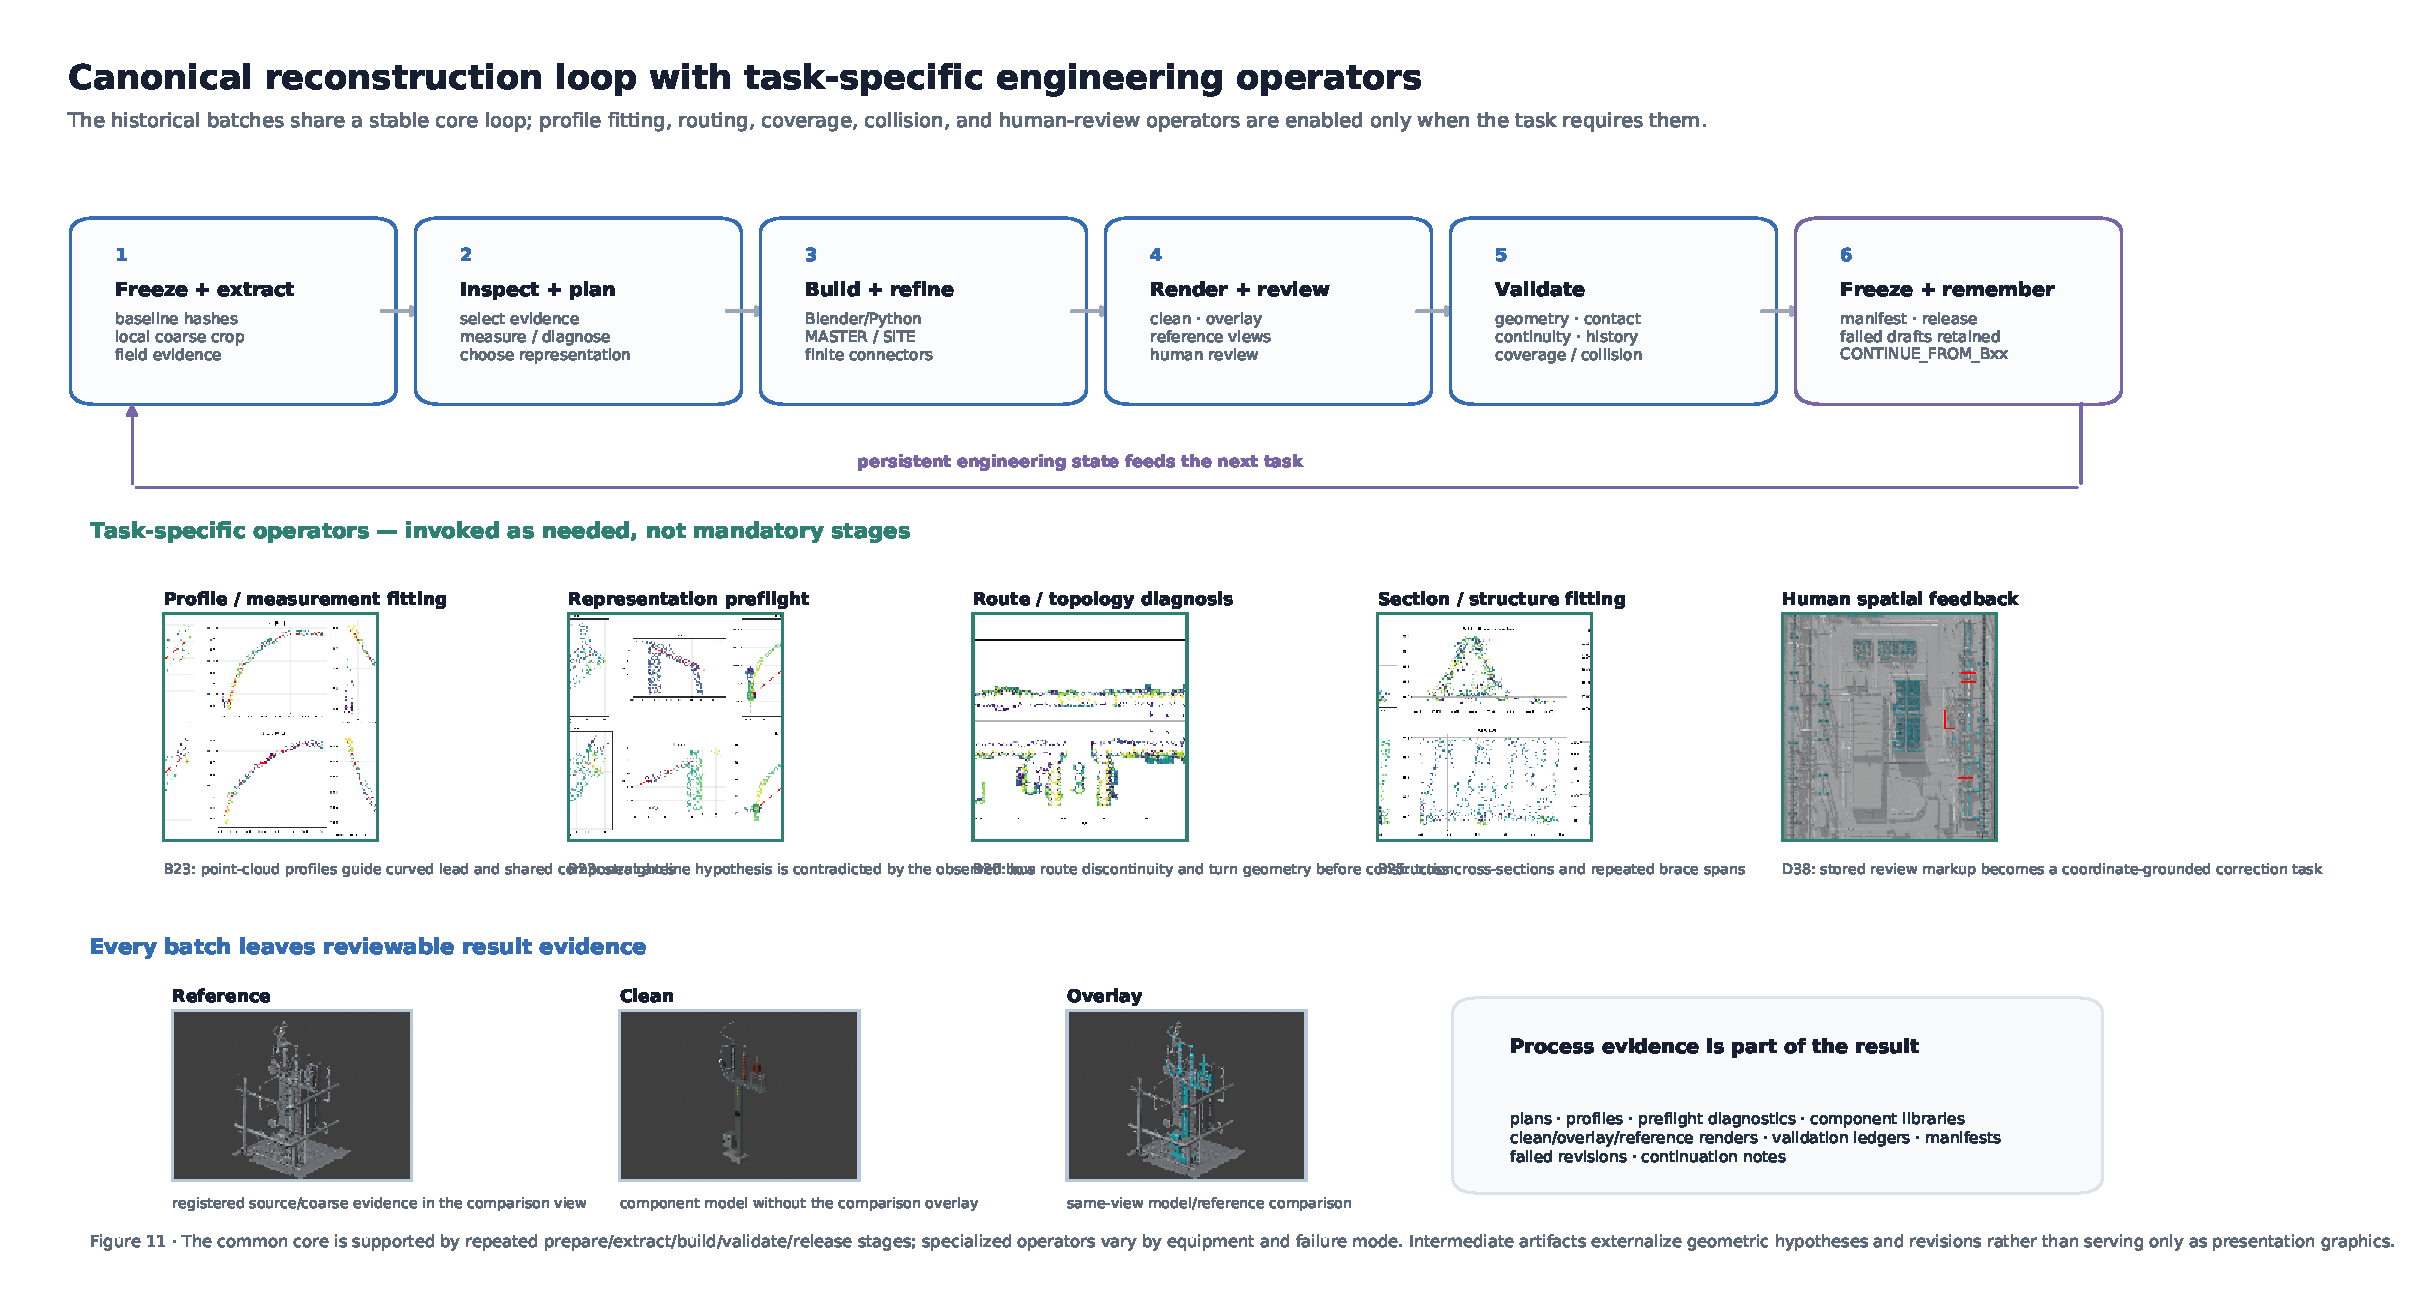
\includegraphics[width=\linewidth]{fig11_canonical_workflow.pdf}
\caption{Canonical reconstruction core plus task-specific engineering operators. Intermediate artifacts externalize the geometric hypothesis being tested rather than serving only as presentation graphics.}
\label{fig:canonical}
\end{figure}

\subsection{Intermediate process evidence}
The output folders preserve the reasoning boundary between evidence and committed geometry. B23, for example, contains point-cloud measurement profiles, a component/lead preflight, a large fitted plan, clean/overlay/reference review triplets, multiple validation/manifests and retained r1/r2/r3 revisions. B20 preserves route diagnostics before bus construction; B25 stores truss profiles and comparison domains; B29 preserves strain, jumper and crossline fits. These artifacts record why a representation was selected, rejected or revised and are exposed in the companion website as per-batch process dossiers.

\subsection{Layered verifier}
\begin{figure}[H]
\centering
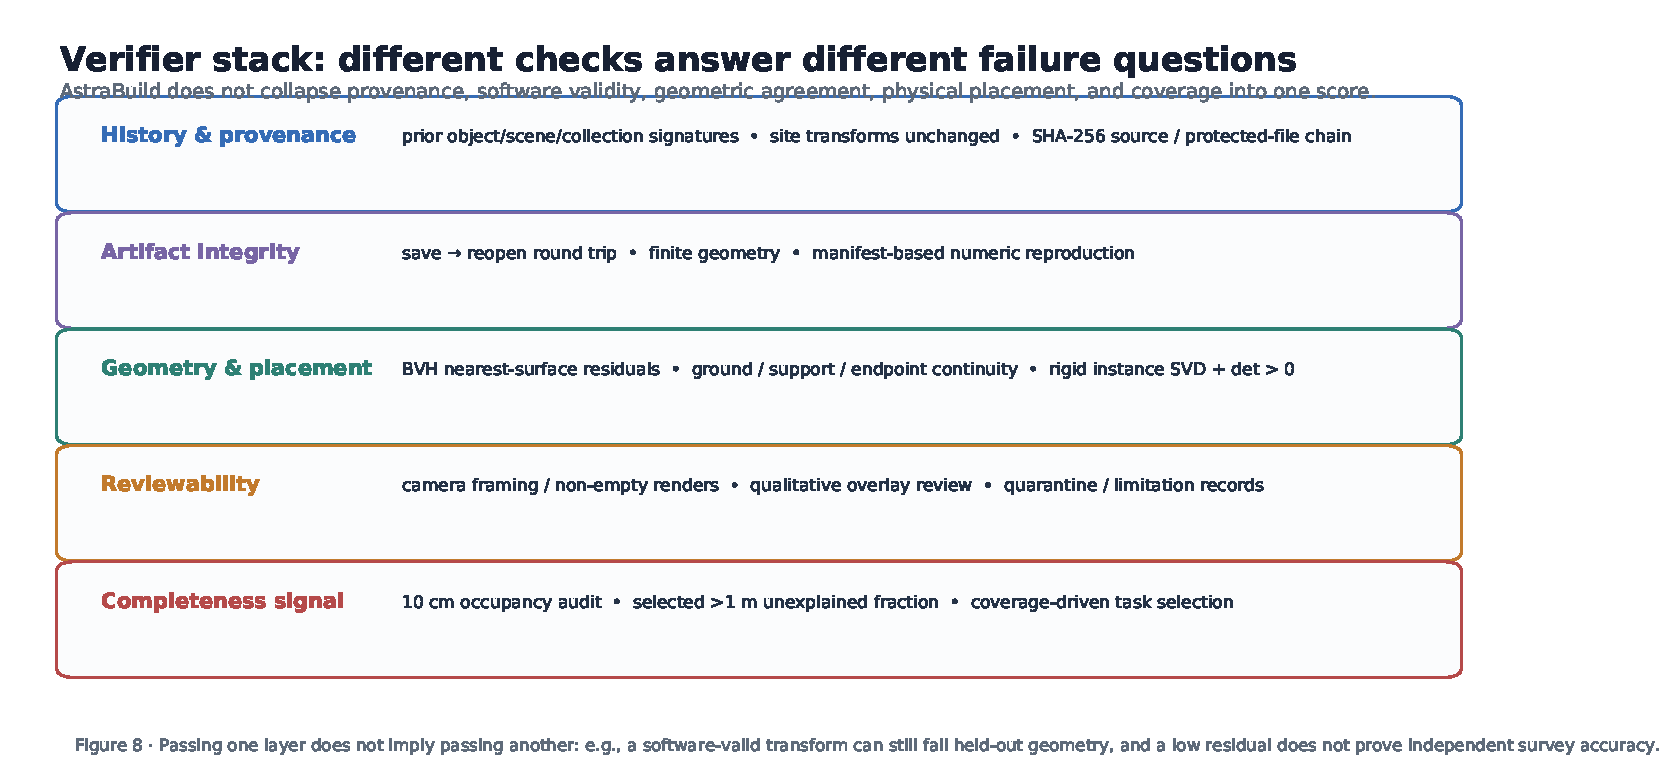
\includegraphics[width=.95\linewidth]{fig08_validation_stack.pdf}
\caption{Validation stack. File validity, history preservation, geometric agreement, placement, reviewability, and coverage answer different questions and are not collapsed into one score.}
\label{fig:verifier}
\end{figure}

\section{Experimental Design and Metrics}
The experiment is longitudinal: later batches inherit earlier geometry and can change the protocol after failure. The record summarizes 38 core batches through D38, 54 builders, 58 validators, 150 manifests, 71 validation JSON files, 28 installation-queue revisions, 109 local reference NPZ crops, and 719 new review scenes. These counts describe an engineering history rather than statistically independent samples.

\begin{figure}[H]
\centering
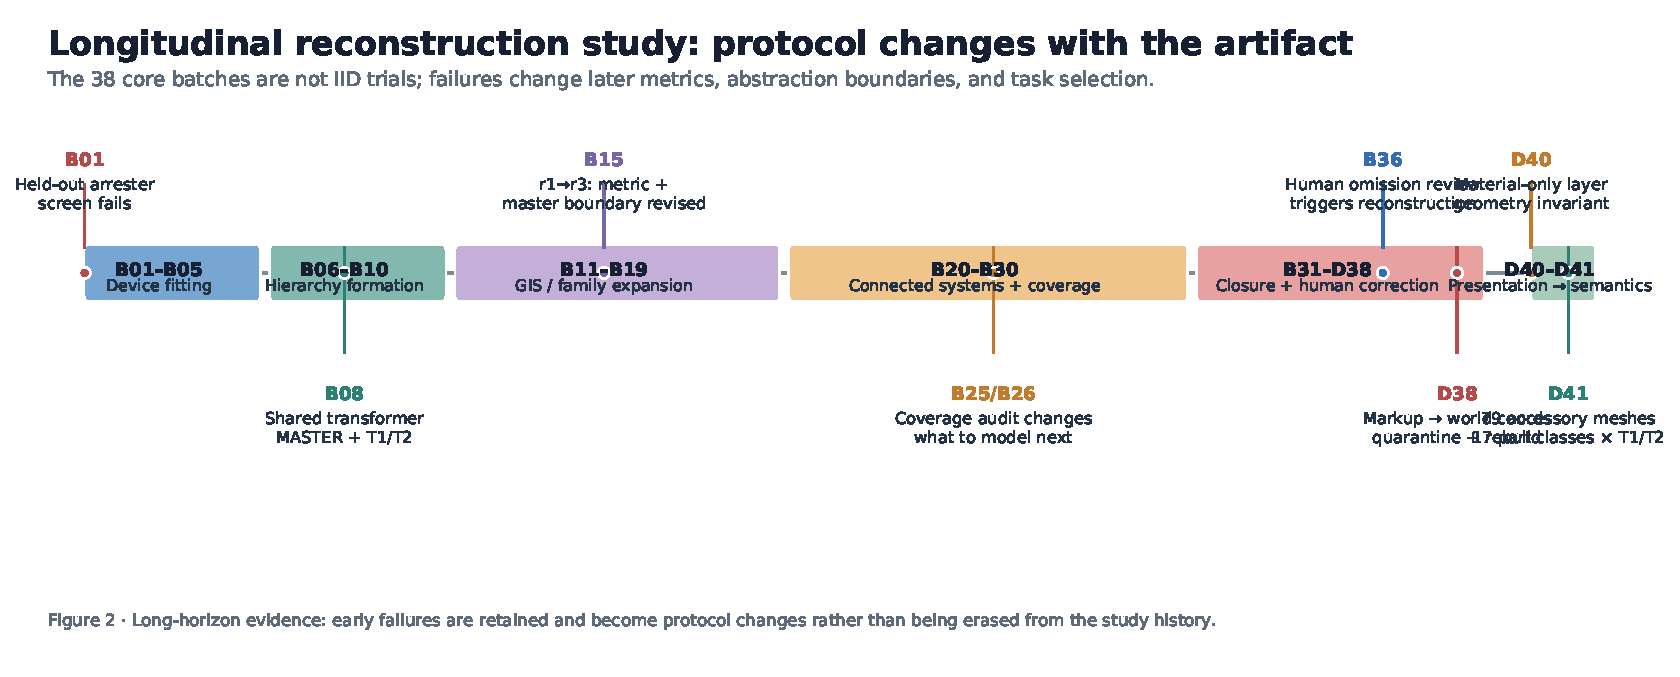
\includegraphics[width=\linewidth]{fig02_longitudinal_study.pdf}
\caption{Longitudinal study phases and protocol-changing events.}
\label{fig:timeline}
\end{figure}

\subsection{Reference-surface residual}
For a retained sample $x_i$ and local reference surface $G$, a generic comparison quantity is
\begin{equation}
d_i=\operatorname{dist}(x_i,G).
\end{equation}
The global summary aggregates heterogeneous current batch records and reports median/p90/p95. \scopewarning{}

\subsection{Five-centimeter screen}
The later report summarizes 149 passing and 101 non-passing retained screen items at a selected 5 cm criterion. This is a validation-screen ledger, not a task success rate.

\subsection{Coverage-gap fraction}
For selected reference samples $\mathcal{P}$ and threshold $\tau=1$~m,
\begin{equation}
C_\tau=\frac{1}{|\mathcal P|}\sum_{p\in\mathcal P}\mathbf 1[\operatorname{dist}(p,M_t)>\tau].
\end{equation}
This is an omission/completeness signal for a selected region, not an absolute reconstruction-accuracy measure.

\subsection{Reuse ratio}
We report the descriptive object/mesh-datablock ratio
\begin{equation}
R_{\text{reuse}}=\frac{37153}{3916}\approx9.5.
\end{equation}
It indicates extensive instancing/shared geometry but is not a labor-speed or storage-compression benchmark.

\section{Results}
\subsection{RQ1: structured scene and reuse}
At the D38.2/D40-equivalent layer, the project contains 37,153 objects, 755 scenes, 858 collections, 3,916 mesh datablocks, and 29,986,649 vertices. The historical report further records 9,022 new root objects over B14--B36 while extensive nested/collection instancing reuses common component geometry.

\subsection{RQ2: reference agreement with explicit non-passing evidence}
The current residual ledger contains $n=1550$ records with median/p90/p95 values 0.036/0.084/0.116~m. A historical pre-fit ledger ($n=450$) has median 0.093~m and large outliers, but the domains/protocol are heterogeneous; it is not a clean stationary before/after distribution. The 5 cm ledger explicitly retains 149 passing and 101 non-passing items.

\subsection{RQ3: coverage-driven completion}
For the selected B25/B26 high-region audit, the fraction of coarse samples farther than 1~m from reconstructed geometry changes from 78.8\% to 14.6\%. Selected GIS220 and transformer high-region medians change from 8.12$\rightarrow$0.15~m and 3.15$\rightarrow$0.06~m respectively. This phase shifts task selection from ``which inventory item remains?'' toward ``which occupied reference region remains unexplained?''

\begin{figure}[H]
\centering
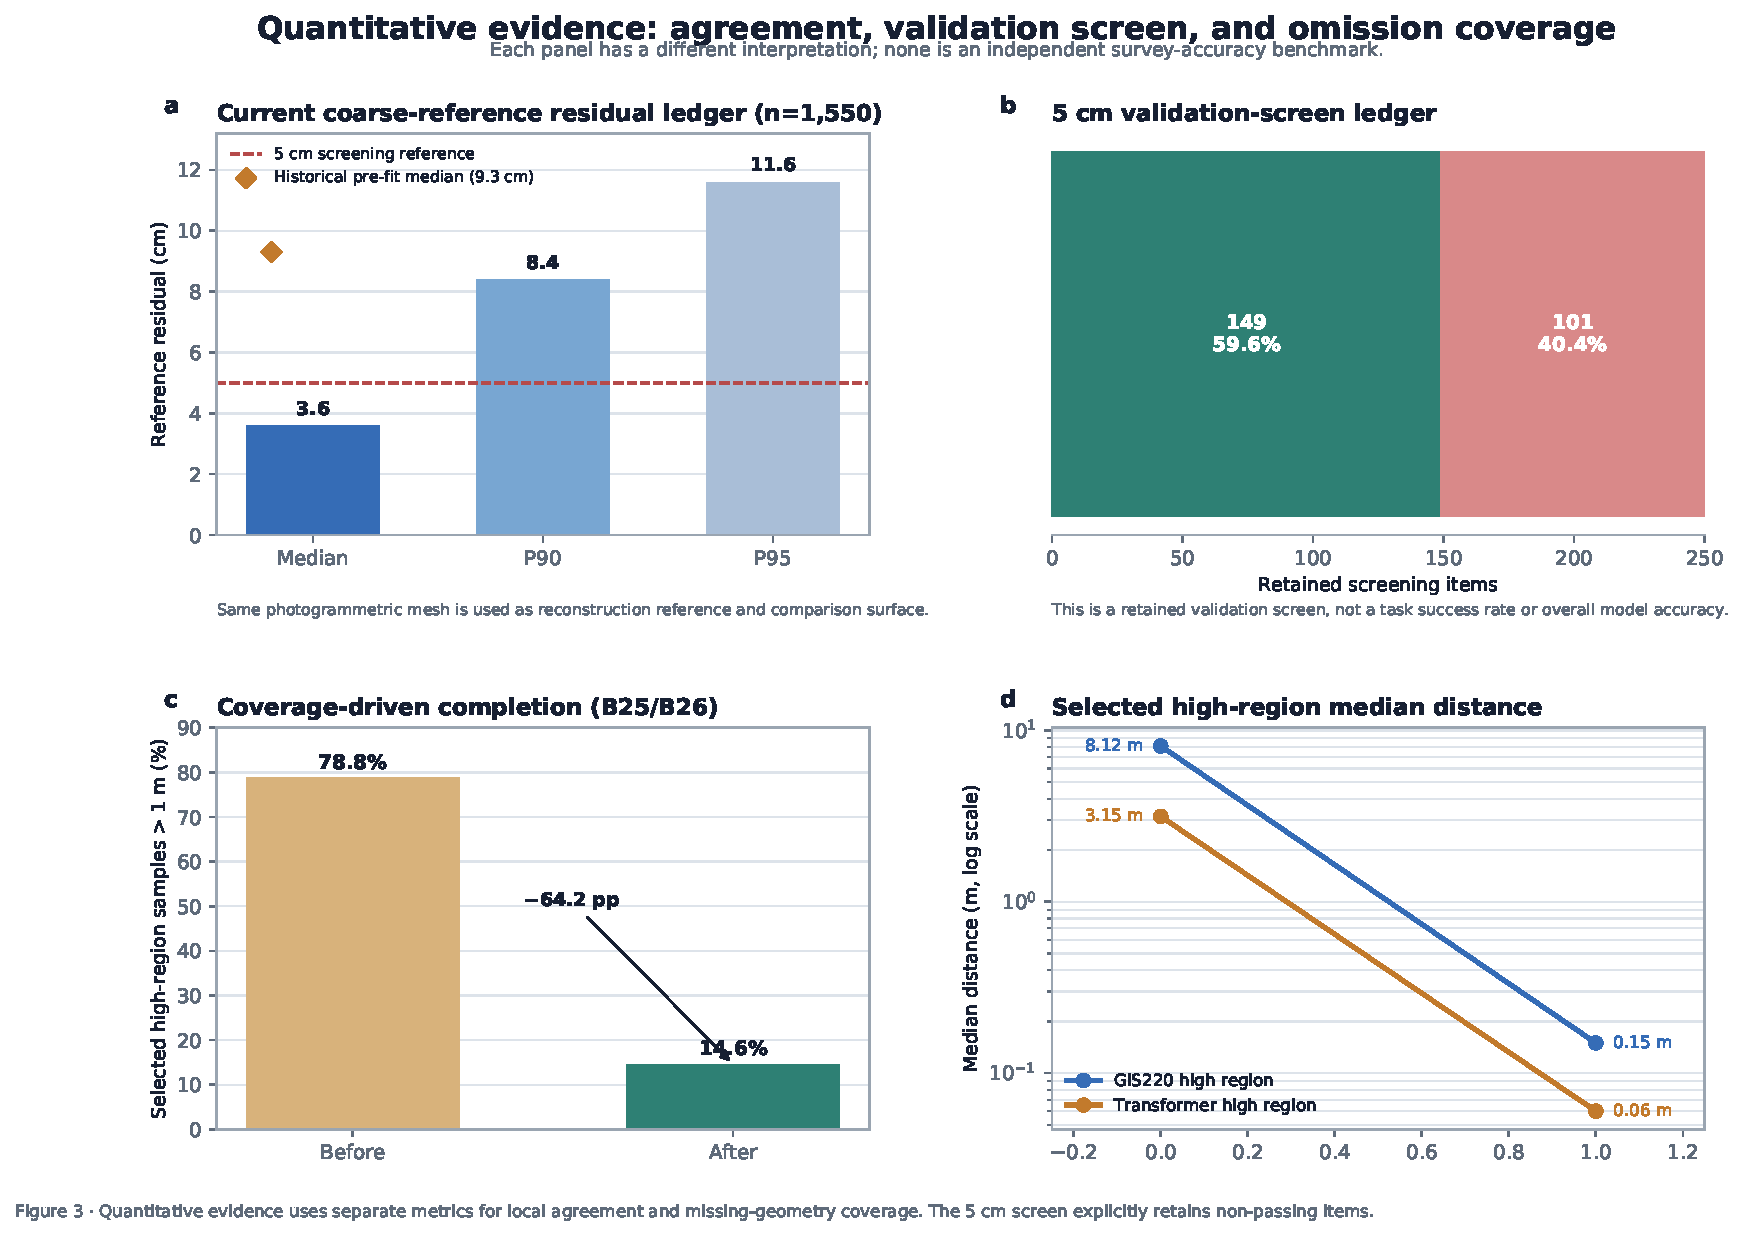
\includegraphics[width=\linewidth]{fig03_quantitative_evidence.pdf}
\caption{Quantitative evidence. Panels intentionally separate local reference agreement, validation-screen status, missing-geometry coverage, and selected high-region before/after distances.}
\label{fig:quant}
\end{figure}

\subsection{RQ1/RQ5: geometry structure and semantic accounting}
The station part map contains 151 devices. Among 106 official names, 76 are attached and 30 remain unmatched. The \#1 transformer pilot maps 189 semantic meshes into 26 part classes. Its 36 official inspection concepts are categorized as 31 model-part, 4 external-component, and 1 non-visual concept.

\begin{figure}[H]
\centering
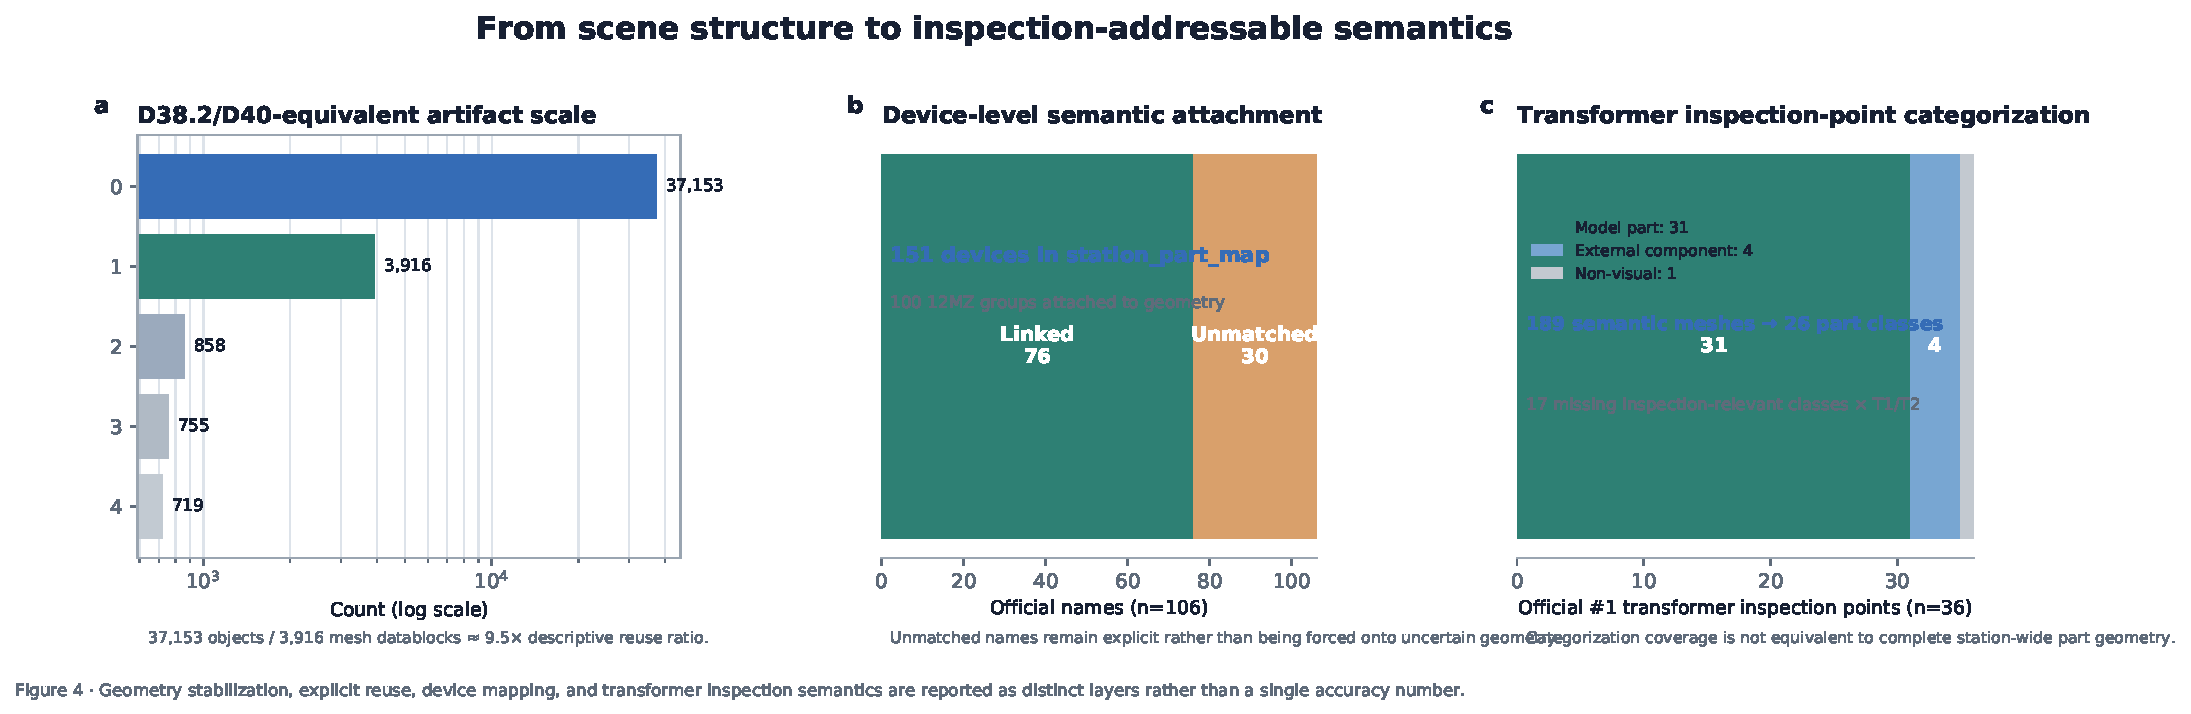
\includegraphics[width=\linewidth]{fig04_structure_and_semantics.pdf}
\caption{Scene structure, device-level semantic attachment, and transformer inspection-point accounting are reported as separate layers.}
\label{fig:semantics}
\end{figure}

\section{Failure and Recovery Studies}
\begin{figure}[H]
\centering
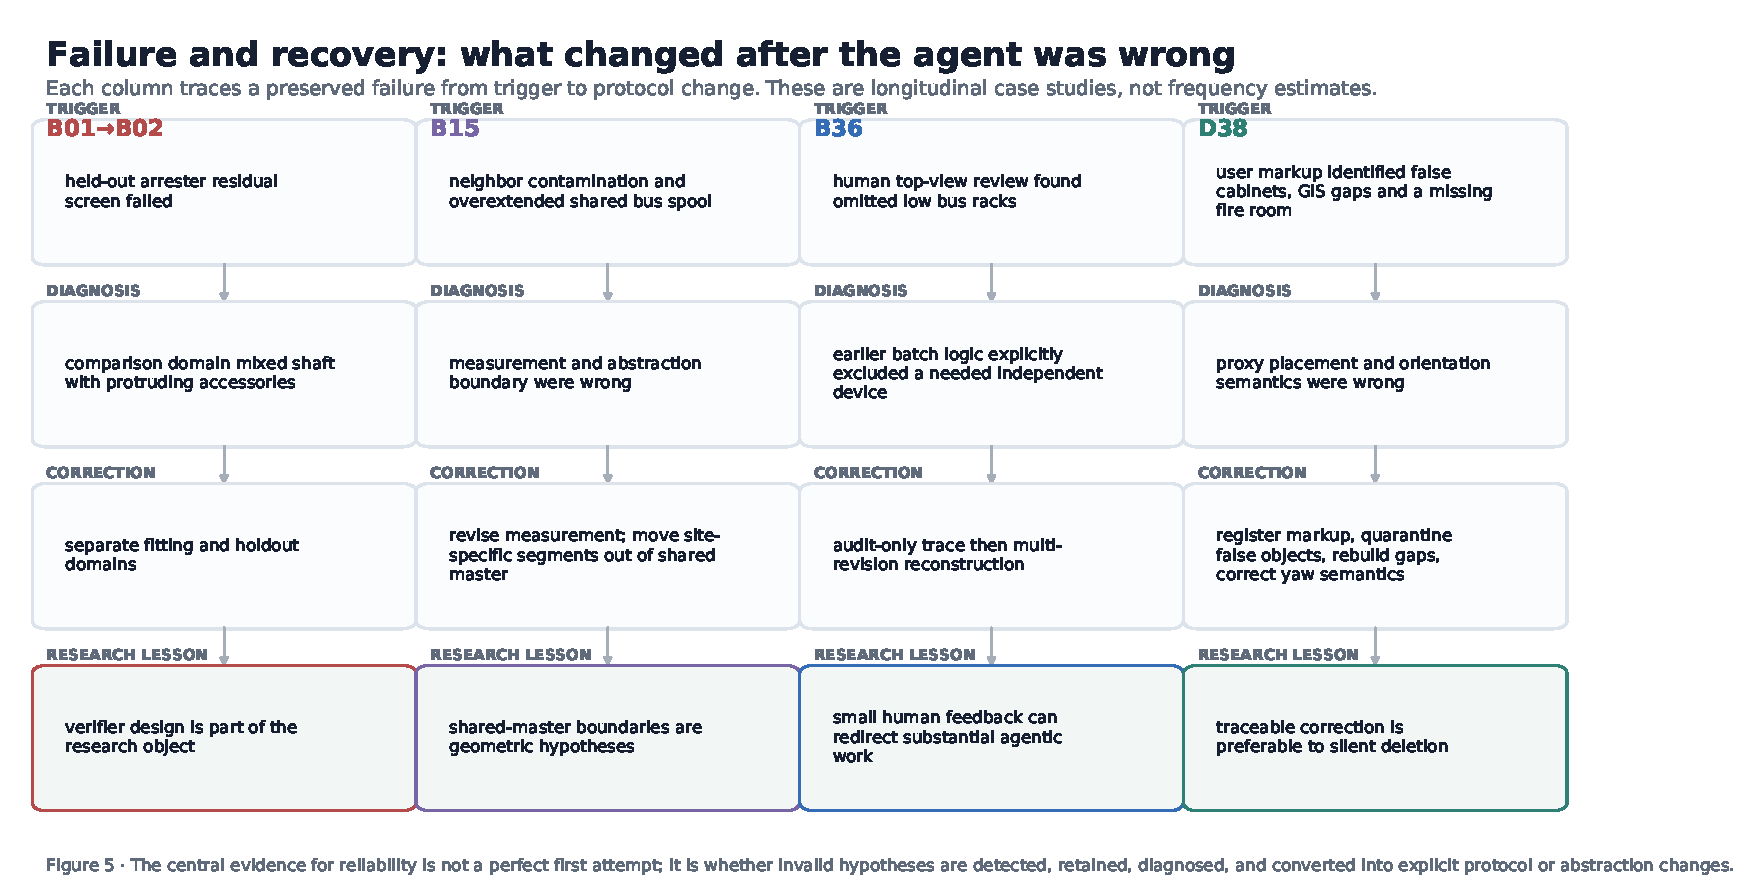
\includegraphics[width=\linewidth]{fig05_failure_recovery.pdf}
\caption{Four preserved failure-to-recovery chains. Each case changes a later measurement, abstraction, or feedback protocol.}
\label{fig:failures}
\end{figure}

\subsection{B01 $\rightarrow$ B02: the verifier changes the metric protocol}
Initial arrester installation passed software-level checks but selected held-out RMS values of approximately 0.048/0.073/0.051~m failed the screen. The batch was preserved; analysis showed that the comparison domain mixed intended shaft geometry with accessory protrusions. B02 separates fitting and holdout domains and explicitly avoids presenting the new metric as a directly comparable improvement.

\subsection{B15: abstraction boundary failure}
Neighbor contamination and an overextended shared bus-spool assumption required multiple revisions. The measurement strategy changed and site-specific finite segments were moved out of the shared master. Component reuse is thus treated as a geometric/equipment hypothesis rather than an unconditional software optimization.

\subsection{B23: process evidence changes the representation}
B23 reconstructs transformer neutral-side mechanisms and leads. An earlier straight-segment preflight does not explain the observed registered coarse geometry, whose mid-span trajectory bows by roughly half a meter. The workflow therefore bins the observed geometry, fits curved control paths, rebuilds the neutral leads and proceeds through retained revisions that add the missing soft connection and lower bridge contact. The final record evaluates 32 fixed comparison domains, with 30 meeting the selected 5~cm screen and two retained misses. The important behavior is representational: measurement/profile evidence changes the class of geometry being built rather than merely adjusting a pose parameter.

\subsection{B36: human review finds omitted geometry}
A top-view reviewer identified missing low transformer-side bus racks. The workflow first audited historical logic, then reconstructed through multiple revisions, preserving an invalid-path draft and later applying a 0.16~m clearance change. Human input supplies the spatial error signal; the agent performs evidence search, code audit, reconstruction, and verification.

\subsection{D38: markup-to-model correction}
Marked review images were registered to stored views (reported normalized correlations 0.94/0.92), inverted to model-world coordinates, and used to diagnose three false cabinet groups, three GIS gaps, and missing fire infrastructure. False objects were quarantined rather than silently deleted. An orientation-semantics error in D38.1 was then caught by overlay review and corrected in D38.2.

\begin{figure}[H]
\centering
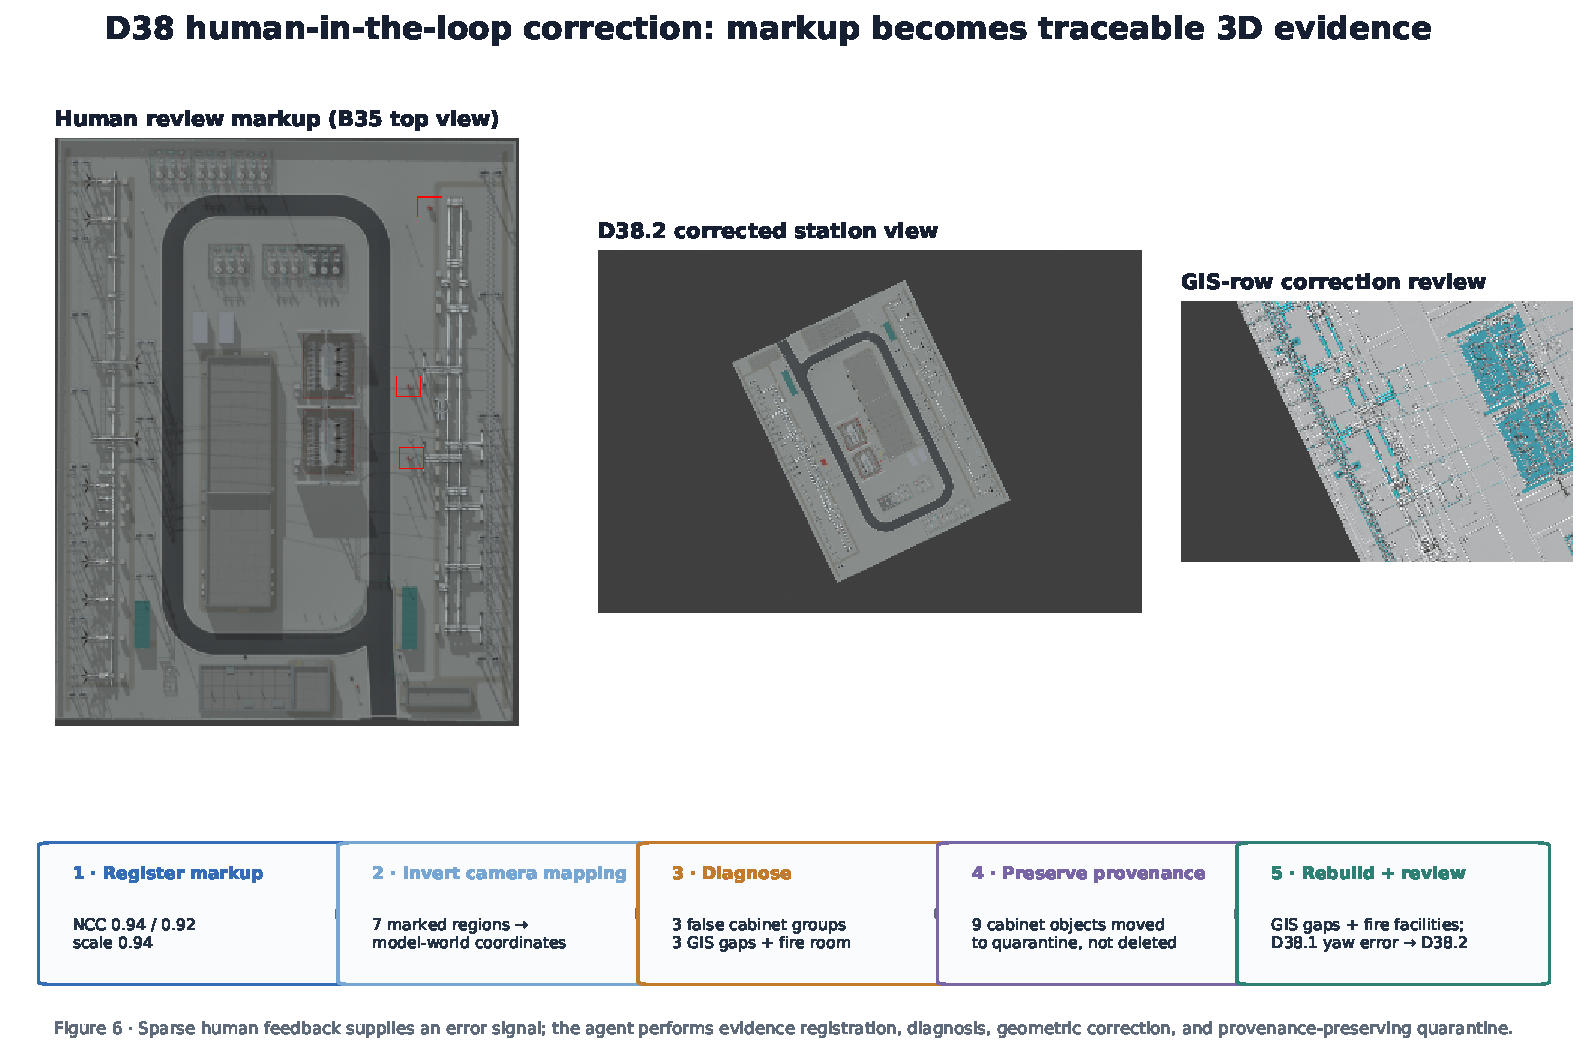
\includegraphics[width=\linewidth]{fig06_d38_human_feedback.pdf}
\caption{D38 human-in-the-loop correction: image markup becomes a traceable sequence of registration, coordinate inference, diagnosis, quarantine/rebuild, and review.}
\label{fig:d38}
\end{figure}

\section{Inspection Semantics and D41}
A later semantic audit shows that identity/part mapping can fail even when geometry is spatially plausible: naming/box heuristics confuse cross-bay bus tubes, arresters, switches, and other nearby components. The v3 semantic pass restructures family rules and explicitly marks missing geometry rather than assigning every record to a nearby object.

D40 provides a useful invariance control: appearance/material assignments are changed while validation checks object/scene/collection/mesh counts, transforms and total vertices against D38. D41 then selects 79 missing transformer accessory meshes spanning 17 inspection-relevant classes and aligns them into a shared accessory collection. The alignment relative to the B08 transformer frame is
\begin{equation}
x'=1.3235x,\quad y'=1.3167y,\quad z'=0.16+1.1567(z-0.45).
\end{equation}
The same accessory master is instantiated for T1 and T2 using the existing site transforms; D41 validation reports \texttt{ok=true} and 79/79 structural checks.

\begin{figure}[H]
\centering
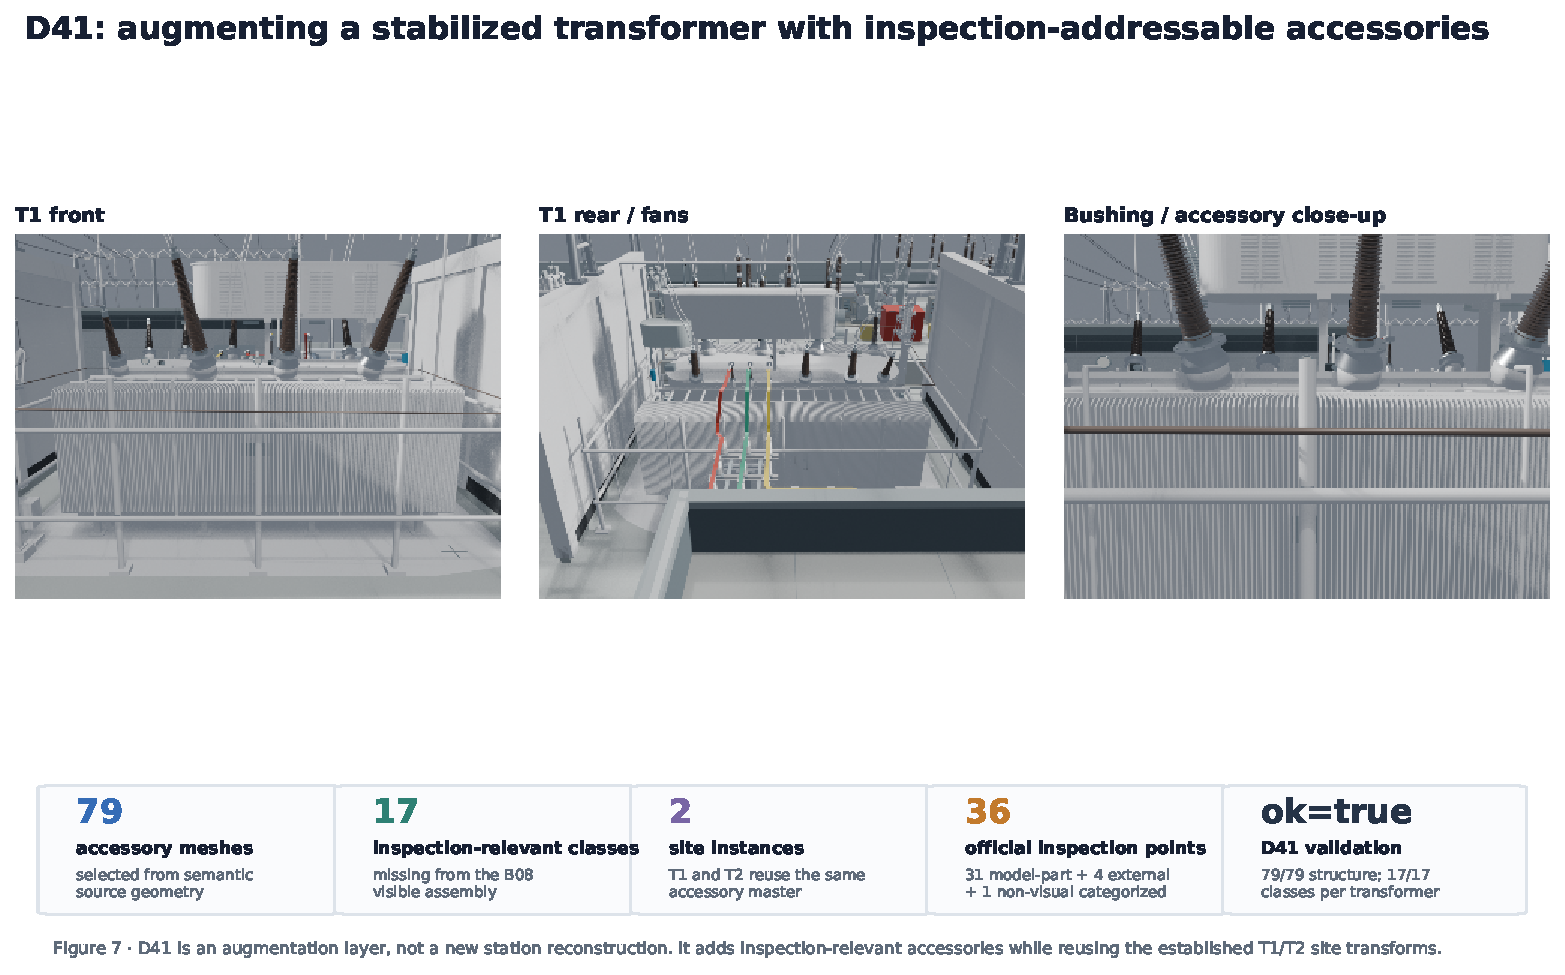
\includegraphics[width=\linewidth]{fig07_d41_inspection_semantics.pdf}
\caption{D41 transformer inspection-semantic augmentation. This is an additive layer on the existing station history, not a new reconstruction baseline.}
\label{fig:d41}
\end{figure}

\section{Discussion}
\paragraph{A reconstruction operator, not a one-shot generator.} The useful behavior is the model's ability to move among evidence, scripts, renders, validators, history, and revised abstractions over a long horizon. This is closer to operating an engineering process than emitting a mesh.

\paragraph{Verification must be heterogeneous.} File validity, reference agreement, placement, coverage and identity are different failure modes. B01 is software-valid but geometry-screen invalid; D38.1 is transformable but orientation-semantics wrong; semantic mappings can be spatially close but identity-wrong.

\paragraph{Reusable components are falsifiable hypotheses.} MASTER/SITE reuse improves consistency only if equivalence is supported. B15 shows why site-specific geometry must sometimes be separated from a shared master.

\paragraph{Coverage becomes a task-selection sensor.} Late-stage occupancy audits identify ``unknown unknowns'' that inventory-driven completion misses, making the coarse mesh useful not only for fitting but for deciding what to inspect/model next.

\paragraph{Human feedback is an interface.} The workflow is agent-driven and human-steerable. Sparse image markup or equivalence approval can redirect large amounts of tool-based work without requiring the reviewer to operate Blender directly.

\section{Limitations and Threats to Validity}
The study covers a single substation and therefore cannot establish cross-site generalization. The headline residuals are not independent survey accuracy because the comparison surface participates in reconstruction. Validation protocols evolve, so the 38 core batches are not IID trials. Historical logs lack matched reruns with other foundation models, lower reasoning effort, or expert CAD operators; thus model-specific causal attribution is not possible. Human intervention materially affects several batches. Old batch logs do not freeze model/reasoning-effort provenance. Several image sets lack complete calibration, hidden components remain inferred, and 30 official names remain unmatched. Finally, request-level token/cost/latency and human-review time are not yet frozen well enough to support resource-efficiency comparisons like those in robot-policy reports.

\section{Conclusion}
AstraBuild suggests a role for general-purpose reasoning in industrial 3D engineering that is broader than direct mesh synthesis. With explicit evidence boundaries, programmatic actuators, layered validation, immutable artifacts, and human-steerable feedback, a model can participate in a persistent reconstruction loop that builds reusable structure, diagnoses failures, changes its own protocol, and connects geometry to later inspection semantics. The next step is a multi-site study with frozen model/tool provenance, independent survey/control-point evaluation, intervention/cost accounting, and controlled model/expert baselines.

\appendix
\section{Version Boundary}
\begin{tabular}{p{0.14\linewidth}p{0.3\linewidth}p{0.47\linewidth}}
\toprule
Layer & Role & Interpretation \\
\midrule
D38.2 & core station geometry after markup correction & principal geometry baseline for headline artifact counts \\
D40 & material/presentation layer & geometry, transforms and vertex counts checked invariant \\
D41 & transformer accessory/inspection layer & additive semantic/geometry augmentation; research endpoint \\
\bottomrule
\end{tabular}

\section{Validation Taxonomy}
The historical report documents recurring checks for history preservation, site transforms, protected hashes, asset round trips, finite geometry, numeric replay, BVH/reference residuals, contact/ground/support continuity, camera framing, rigid-instance SVD, and occupancy/coverage auditing. A future release should encode these checks in a stable versioned schema rather than relying on partially heterogeneous batch JSON structures.

\section{Claim Guardrails}
\begin{itemize}
\item Allowed: ``median residual to the same photogrammetric reference mesh is 3.6 cm.'' Not allowed: ``absolute reconstruction accuracy is 3.6 cm.''
\item Allowed: ``149/250 retained 5 cm screening items pass.'' Not allowed: ``the model has 59.6\% accuracy.''
\item Allowed: ``selected high-region $>1$ m gap fraction changes 78.8\%$\rightarrow$14.6\%.'' Not allowed: ``whole-station completeness is 85.4\%.''
\item Allowed: ``the workflow is agent-driven and human-steerable.'' Not allowed: ``the station was reconstructed fully autonomously.''
\end{itemize}

\bibliographystyle{plain}
\bibliography{references}
\end{document}
